
\documentclass{article} % For LaTeX2e
\usepackage{iclr2020_conference,times,natbib}

% Optional math commands from https://github.com/goodfeli/dlbook_notation.
%%%%% NEW MATH DEFINITIONS %%%%%

\usepackage{amsmath,amsfonts,bm}

% Mark sections of captions for referring to divisions of figures
\newcommand{\figleft}{{\em (Left)}}
\newcommand{\figcenter}{{\em (Center)}}
\newcommand{\figright}{{\em (Right)}}
\newcommand{\figtop}{{\em (Top)}}
\newcommand{\figbottom}{{\em (Bottom)}}
\newcommand{\captiona}{{\em (a)}}
\newcommand{\captionb}{{\em (b)}}
\newcommand{\captionc}{{\em (c)}}
\newcommand{\captiond}{{\em (d)}}

% Highlight a newly defined term
\newcommand{\newterm}[1]{{\bf #1}}


% Figure reference, lower-case.
\def\figref#1{figure~\ref{#1}}
% Figure reference, capital. For start of sentence
\def\Figref#1{Figure~\ref{#1}}
\def\twofigref#1#2{figures \ref{#1} and \ref{#2}}
\def\quadfigref#1#2#3#4{figures \ref{#1}, \ref{#2}, \ref{#3} and \ref{#4}}
% Section reference, lower-case.
\def\secref#1{section~\ref{#1}}
% Section reference, capital.
\def\Secref#1{Section~\ref{#1}}
% Reference to two sections.
\def\twosecrefs#1#2{sections \ref{#1} and \ref{#2}}
% Reference to three sections.
\def\secrefs#1#2#3{sections \ref{#1}, \ref{#2} and \ref{#3}}
% Reference to an equation, lower-case.
\def\eqref#1{equation~\ref{#1}}
% Reference to an equation, upper case
\def\Eqref#1{Equation~\ref{#1}}
% A raw reference to an equation---avoid using if possible
\def\plaineqref#1{\ref{#1}}
% Reference to a chapter, lower-case.
\def\chapref#1{chapter~\ref{#1}}
% Reference to an equation, upper case.
\def\Chapref#1{Chapter~\ref{#1}}
% Reference to a range of chapters
\def\rangechapref#1#2{chapters\ref{#1}--\ref{#2}}
% Reference to an algorithm, lower-case.
\def\algref#1{algorithm~\ref{#1}}
% Reference to an algorithm, upper case.
\def\Algref#1{Algorithm~\ref{#1}}
\def\twoalgref#1#2{algorithms \ref{#1} and \ref{#2}}
\def\Twoalgref#1#2{Algorithms \ref{#1} and \ref{#2}}
% Reference to a part, lower case
\def\partref#1{part~\ref{#1}}
% Reference to a part, upper case
\def\Partref#1{Part~\ref{#1}}
\def\twopartref#1#2{parts \ref{#1} and \ref{#2}}

\def\ceil#1{\lceil #1 \rceil}
\def\floor#1{\lfloor #1 \rfloor}
\def\1{\bm{1}}
\newcommand{\train}{\mathcal{D}}
\newcommand{\valid}{\mathcal{D_{\mathrm{valid}}}}
\newcommand{\test}{\mathcal{D_{\mathrm{test}}}}

\def\eps{{\epsilon}}


% Random variables
\def\reta{{\textnormal{$\eta$}}}
\def\ra{{\textnormal{a}}}
\def\rb{{\textnormal{b}}}
\def\rc{{\textnormal{c}}}
\def\rd{{\textnormal{d}}}
\def\re{{\textnormal{e}}}
\def\rf{{\textnormal{f}}}
\def\rg{{\textnormal{g}}}
\def\rh{{\textnormal{h}}}
\def\ri{{\textnormal{i}}}
\def\rj{{\textnormal{j}}}
\def\rk{{\textnormal{k}}}
\def\rl{{\textnormal{l}}}
% rm is already a command, just don't name any random variables m
\def\rn{{\textnormal{n}}}
\def\ro{{\textnormal{o}}}
\def\rp{{\textnormal{p}}}
\def\rq{{\textnormal{q}}}
\def\rr{{\textnormal{r}}}
\def\rs{{\textnormal{s}}}
\def\rt{{\textnormal{t}}}
\def\ru{{\textnormal{u}}}
\def\rv{{\textnormal{v}}}
\def\rw{{\textnormal{w}}}
\def\rx{{\textnormal{x}}}
\def\ry{{\textnormal{y}}}
\def\rz{{\textnormal{z}}}

% Random vectors
\def\rvepsilon{{\mathbf{\epsilon}}}
\def\rvtheta{{\mathbf{\theta}}}
\def\rva{{\mathbf{a}}}
\def\rvb{{\mathbf{b}}}
\def\rvc{{\mathbf{c}}}
\def\rvd{{\mathbf{d}}}
\def\rve{{\mathbf{e}}}
\def\rvf{{\mathbf{f}}}
\def\rvg{{\mathbf{g}}}
\def\rvh{{\mathbf{h}}}
\def\rvu{{\mathbf{i}}}
\def\rvj{{\mathbf{j}}}
\def\rvk{{\mathbf{k}}}
\def\rvl{{\mathbf{l}}}
\def\rvm{{\mathbf{m}}}
\def\rvn{{\mathbf{n}}}
\def\rvo{{\mathbf{o}}}
\def\rvp{{\mathbf{p}}}
\def\rvq{{\mathbf{q}}}
\def\rvr{{\mathbf{r}}}
\def\rvs{{\mathbf{s}}}
\def\rvt{{\mathbf{t}}}
\def\rvu{{\mathbf{u}}}
\def\rvv{{\mathbf{v}}}
\def\rvw{{\mathbf{w}}}
\def\rvx{{\mathbf{x}}}
\def\rvy{{\mathbf{y}}}
\def\rvz{{\mathbf{z}}}

% Elements of random vectors
\def\erva{{\textnormal{a}}}
\def\ervb{{\textnormal{b}}}
\def\ervc{{\textnormal{c}}}
\def\ervd{{\textnormal{d}}}
\def\erve{{\textnormal{e}}}
\def\ervf{{\textnormal{f}}}
\def\ervg{{\textnormal{g}}}
\def\ervh{{\textnormal{h}}}
\def\ervi{{\textnormal{i}}}
\def\ervj{{\textnormal{j}}}
\def\ervk{{\textnormal{k}}}
\def\ervl{{\textnormal{l}}}
\def\ervm{{\textnormal{m}}}
\def\ervn{{\textnormal{n}}}
\def\ervo{{\textnormal{o}}}
\def\ervp{{\textnormal{p}}}
\def\ervq{{\textnormal{q}}}
\def\ervr{{\textnormal{r}}}
\def\ervs{{\textnormal{s}}}
\def\ervt{{\textnormal{t}}}
\def\ervu{{\textnormal{u}}}
\def\ervv{{\textnormal{v}}}
\def\ervw{{\textnormal{w}}}
\def\ervx{{\textnormal{x}}}
\def\ervy{{\textnormal{y}}}
\def\ervz{{\textnormal{z}}}

% Random matrices
\def\rmA{{\mathbf{A}}}
\def\rmB{{\mathbf{B}}}
\def\rmC{{\mathbf{C}}}
\def\rmD{{\mathbf{D}}}
\def\rmE{{\mathbf{E}}}
\def\rmF{{\mathbf{F}}}
\def\rmG{{\mathbf{G}}}
\def\rmH{{\mathbf{H}}}
\def\rmI{{\mathbf{I}}}
\def\rmJ{{\mathbf{J}}}
\def\rmK{{\mathbf{K}}}
\def\rmL{{\mathbf{L}}}
\def\rmM{{\mathbf{M}}}
\def\rmN{{\mathbf{N}}}
\def\rmO{{\mathbf{O}}}
\def\rmP{{\mathbf{P}}}
\def\rmQ{{\mathbf{Q}}}
\def\rmR{{\mathbf{R}}}
\def\rmS{{\mathbf{S}}}
\def\rmT{{\mathbf{T}}}
\def\rmU{{\mathbf{U}}}
\def\rmV{{\mathbf{V}}}
\def\rmW{{\mathbf{W}}}
\def\rmX{{\mathbf{X}}}
\def\rmY{{\mathbf{Y}}}
\def\rmZ{{\mathbf{Z}}}

% Elements of random matrices
\def\ermA{{\textnormal{A}}}
\def\ermB{{\textnormal{B}}}
\def\ermC{{\textnormal{C}}}
\def\ermD{{\textnormal{D}}}
\def\ermE{{\textnormal{E}}}
\def\ermF{{\textnormal{F}}}
\def\ermG{{\textnormal{G}}}
\def\ermH{{\textnormal{H}}}
\def\ermI{{\textnormal{I}}}
\def\ermJ{{\textnormal{J}}}
\def\ermK{{\textnormal{K}}}
\def\ermL{{\textnormal{L}}}
\def\ermM{{\textnormal{M}}}
\def\ermN{{\textnormal{N}}}
\def\ermO{{\textnormal{O}}}
\def\ermP{{\textnormal{P}}}
\def\ermQ{{\textnormal{Q}}}
\def\ermR{{\textnormal{R}}}
\def\ermS{{\textnormal{S}}}
\def\ermT{{\textnormal{T}}}
\def\ermU{{\textnormal{U}}}
\def\ermV{{\textnormal{V}}}
\def\ermW{{\textnormal{W}}}
\def\ermX{{\textnormal{X}}}
\def\ermY{{\textnormal{Y}}}
\def\ermZ{{\textnormal{Z}}}

% Vectors
\def\vzero{{\bm{0}}}
\def\vone{{\bm{1}}}
\def\vmu{{\bm{\mu}}}
\def\vtheta{{\bm{\theta}}}
\def\va{{\bm{a}}}
\def\vb{{\bm{b}}}
\def\vc{{\bm{c}}}
\def\vd{{\bm{d}}}
\def\ve{{\bm{e}}}
\def\vf{{\bm{f}}}
\def\vg{{\bm{g}}}
\def\vh{{\bm{h}}}
\def\vi{{\bm{i}}}
\def\vj{{\bm{j}}}
\def\vk{{\bm{k}}}
\def\vl{{\bm{l}}}
\def\vm{{\bm{m}}}
\def\vn{{\bm{n}}}
\def\vo{{\bm{o}}}
\def\vp{{\bm{p}}}
\def\vq{{\bm{q}}}
\def\vr{{\bm{r}}}
\def\vs{{\bm{s}}}
\def\vt{{\bm{t}}}
\def\vu{{\bm{u}}}
\def\vv{{\bm{v}}}
\def\vw{{\bm{w}}}
\def\vx{{\bm{x}}}
\def\vy{{\bm{y}}}
\def\vz{{\bm{z}}}

% Elements of vectors
\def\evalpha{{\alpha}}
\def\evbeta{{\beta}}
\def\evepsilon{{\epsilon}}
\def\evlambda{{\lambda}}
\def\evomega{{\omega}}
\def\evmu{{\mu}}
\def\evpsi{{\psi}}
\def\evsigma{{\sigma}}
\def\evtheta{{\theta}}
\def\eva{{a}}
\def\evb{{b}}
\def\evc{{c}}
\def\evd{{d}}
\def\eve{{e}}
\def\evf{{f}}
\def\evg{{g}}
\def\evh{{h}}
\def\evi{{i}}
\def\evj{{j}}
\def\evk{{k}}
\def\evl{{l}}
\def\evm{{m}}
\def\evn{{n}}
\def\evo{{o}}
\def\evp{{p}}
\def\evq{{q}}
\def\evr{{r}}
\def\evs{{s}}
\def\evt{{t}}
\def\evu{{u}}
\def\evv{{v}}
\def\evw{{w}}
\def\evx{{x}}
\def\evy{{y}}
\def\evz{{z}}

% Matrix
\def\mA{{\bm{A}}}
\def\mB{{\bm{B}}}
\def\mC{{\bm{C}}}
\def\mD{{\bm{D}}}
\def\mE{{\bm{E}}}
\def\mF{{\bm{F}}}
\def\mG{{\bm{G}}}
\def\mH{{\bm{H}}}
\def\mI{{\bm{I}}}
\def\mJ{{\bm{J}}}
\def\mK{{\bm{K}}}
\def\mL{{\bm{L}}}
\def\mM{{\bm{M}}}
\def\mN{{\bm{N}}}
\def\mO{{\bm{O}}}
\def\mP{{\bm{P}}}
\def\mQ{{\bm{Q}}}
\def\mR{{\bm{R}}}
\def\mS{{\bm{S}}}
\def\mT{{\bm{T}}}
\def\mU{{\bm{U}}}
\def\mV{{\bm{V}}}
\def\mW{{\bm{W}}}
\def\mX{{\bm{X}}}
\def\mY{{\bm{Y}}}
\def\mZ{{\bm{Z}}}
\def\mBeta{{\bm{\beta}}}
\def\mPhi{{\bm{\Phi}}}
\def\mLambda{{\bm{\Lambda}}}
\def\mSigma{{\bm{\Sigma}}}

% Tensor
\DeclareMathAlphabet{\mathsfit}{\encodingdefault}{\sfdefault}{m}{sl}
\SetMathAlphabet{\mathsfit}{bold}{\encodingdefault}{\sfdefault}{bx}{n}
\newcommand{\tens}[1]{\bm{\mathsfit{#1}}}
\def\tA{{\tens{A}}}
\def\tB{{\tens{B}}}
\def\tC{{\tens{C}}}
\def\tD{{\tens{D}}}
\def\tE{{\tens{E}}}
\def\tF{{\tens{F}}}
\def\tG{{\tens{G}}}
\def\tH{{\tens{H}}}
\def\tI{{\tens{I}}}
\def\tJ{{\tens{J}}}
\def\tK{{\tens{K}}}
\def\tL{{\tens{L}}}
\def\tM{{\tens{M}}}
\def\tN{{\tens{N}}}
\def\tO{{\tens{O}}}
\def\tP{{\tens{P}}}
\def\tQ{{\tens{Q}}}
\def\tR{{\tens{R}}}
\def\tS{{\tens{S}}}
\def\tT{{\tens{T}}}
\def\tU{{\tens{U}}}
\def\tV{{\tens{V}}}
\def\tW{{\tens{W}}}
\def\tX{{\tens{X}}}
\def\tY{{\tens{Y}}}
\def\tZ{{\tens{Z}}}


% Graph
\def\gA{{\mathcal{A}}}
\def\gB{{\mathcal{B}}}
\def\gC{{\mathcal{C}}}
\def\gD{{\mathcal{D}}}
\def\gE{{\mathcal{E}}}
\def\gF{{\mathcal{F}}}
\def\gG{{\mathcal{G}}}
\def\gH{{\mathcal{H}}}
\def\gI{{\mathcal{I}}}
\def\gJ{{\mathcal{J}}}
\def\gK{{\mathcal{K}}}
\def\gL{{\mathcal{L}}}
\def\gM{{\mathcal{M}}}
\def\gN{{\mathcal{N}}}
\def\gO{{\mathcal{O}}}
\def\gP{{\mathcal{P}}}
\def\gQ{{\mathcal{Q}}}
\def\gR{{\mathcal{R}}}
\def\gS{{\mathcal{S}}}
\def\gT{{\mathcal{T}}}
\def\gU{{\mathcal{U}}}
\def\gV{{\mathcal{V}}}
\def\gW{{\mathcal{W}}}
\def\gX{{\mathcal{X}}}
\def\gY{{\mathcal{Y}}}
\def\gZ{{\mathcal{Z}}}

% Sets
\def\sA{{\mathbb{A}}}
\def\sB{{\mathbb{B}}}
\def\sC{{\mathbb{C}}}
\def\sD{{\mathbb{D}}}
% Don't use a set called E, because this would be the same as our symbol
% for expectation.
\def\sF{{\mathbb{F}}}
\def\sG{{\mathbb{G}}}
\def\sH{{\mathbb{H}}}
\def\sI{{\mathbb{I}}}
\def\sJ{{\mathbb{J}}}
\def\sK{{\mathbb{K}}}
\def\sL{{\mathbb{L}}}
\def\sM{{\mathbb{M}}}
\def\sN{{\mathbb{N}}}
\def\sO{{\mathbb{O}}}
\def\sP{{\mathbb{P}}}
\def\sQ{{\mathbb{Q}}}
\def\sR{{\mathbb{R}}}
\def\sS{{\mathbb{S}}}
\def\sT{{\mathbb{T}}}
\def\sU{{\mathbb{U}}}
\def\sV{{\mathbb{V}}}
\def\sW{{\mathbb{W}}}
\def\sX{{\mathbb{X}}}
\def\sY{{\mathbb{Y}}}
\def\sZ{{\mathbb{Z}}}

% Entries of a matrix
\def\emLambda{{\Lambda}}
\def\emA{{A}}
\def\emB{{B}}
\def\emC{{C}}
\def\emD{{D}}
\def\emE{{E}}
\def\emF{{F}}
\def\emG{{G}}
\def\emH{{H}}
\def\emI{{I}}
\def\emJ{{J}}
\def\emK{{K}}
\def\emL{{L}}
\def\emM{{M}}
\def\emN{{N}}
\def\emO{{O}}
\def\emP{{P}}
\def\emQ{{Q}}
\def\emR{{R}}
\def\emS{{S}}
\def\emT{{T}}
\def\emU{{U}}
\def\emV{{V}}
\def\emW{{W}}
\def\emX{{X}}
\def\emY{{Y}}
\def\emZ{{Z}}
\def\emSigma{{\Sigma}}

% entries of a tensor
% Same font as tensor, without \bm wrapper
\newcommand{\etens}[1]{\mathsfit{#1}}
\def\etLambda{{\etens{\Lambda}}}
\def\etA{{\etens{A}}}
\def\etB{{\etens{B}}}
\def\etC{{\etens{C}}}
\def\etD{{\etens{D}}}
\def\etE{{\etens{E}}}
\def\etF{{\etens{F}}}
\def\etG{{\etens{G}}}
\def\etH{{\etens{H}}}
\def\etI{{\etens{I}}}
\def\etJ{{\etens{J}}}
\def\etK{{\etens{K}}}
\def\etL{{\etens{L}}}
\def\etM{{\etens{M}}}
\def\etN{{\etens{N}}}
\def\etO{{\etens{O}}}
\def\etP{{\etens{P}}}
\def\etQ{{\etens{Q}}}
\def\etR{{\etens{R}}}
\def\etS{{\etens{S}}}
\def\etT{{\etens{T}}}
\def\etU{{\etens{U}}}
\def\etV{{\etens{V}}}
\def\etW{{\etens{W}}}
\def\etX{{\etens{X}}}
\def\etY{{\etens{Y}}}
\def\etZ{{\etens{Z}}}

% The true underlying data generating distribution
\newcommand{\pdata}{p_{\rm{data}}}
% The empirical distribution defined by the training set
\newcommand{\ptrain}{\hat{p}_{\rm{data}}}
\newcommand{\Ptrain}{\hat{P}_{\rm{data}}}
% The model distribution
\newcommand{\pmodel}{p_{\rm{model}}}
\newcommand{\Pmodel}{P_{\rm{model}}}
\newcommand{\ptildemodel}{\tilde{p}_{\rm{model}}}
% Stochastic autoencoder distributions
\newcommand{\pencode}{p_{\rm{encoder}}}
\newcommand{\pdecode}{p_{\rm{decoder}}}
\newcommand{\precons}{p_{\rm{reconstruct}}}

\newcommand{\laplace}{\mathrm{Laplace}} % Laplace distribution

\newcommand{\E}{\mathbb{E}}
\newcommand{\Ls}{\mathcal{L}}
\newcommand{\R}{\mathbb{R}}
\newcommand{\emp}{\tilde{p}}
\newcommand{\lr}{\alpha}
\newcommand{\reg}{\lambda}
\newcommand{\rect}{\mathrm{rectifier}}
\newcommand{\softmax}{\mathrm{softmax}}
\newcommand{\sigmoid}{\sigma}
\newcommand{\softplus}{\zeta}
\newcommand{\KL}{D_{\mathrm{KL}}}
\newcommand{\Var}{\mathrm{Var}}
\newcommand{\standarderror}{\mathrm{SE}}
\newcommand{\Cov}{\mathrm{Cov}}
% Wolfram Mathworld says $L^2$ is for function spaces and $\ell^2$ is for vectors
% But then they seem to use $L^2$ for vectors throughout the site, and so does
% wikipedia.
\newcommand{\normlzero}{L^0}
\newcommand{\normlone}{L^1}
\newcommand{\normltwo}{L^2}
\newcommand{\normlp}{L^p}
\newcommand{\normmax}{L^\infty}

\newcommand{\parents}{Pa} % See usage in notation.tex. Chosen to match Daphne's book.

\DeclareMathOperator*{\argmax}{arg\,max}
\DeclareMathOperator*{\argmin}{arg\,min}

\DeclareMathOperator{\sign}{sign}
\DeclareMathOperator{\Tr}{Tr}
\let\ab\allowbreak


\usepackage[hyphens,spaces,obeyspaces]{url}
\usepackage{hyperref}
\iclrfinalcopy
\usepackage{array}
\usepackage{graphicx} 
\usepackage{float} 
\usepackage{subfigure} 
%\renewcommand{\arraystretch}{1.5}

\title{Instrumental audio synthesis using GANs \\ Progress Report}

% Authors must not appear in the submitted version. They should be hidden
% as long as the \iclrfinalcopy macro remains commented out below.
% Non-anonymous submissions will be rejected without review.

\author{Group N\\Etienne Leclerc (V00853992), Jordie Shier (V00688891), Lu Lu (V00836042),\\ Yangruirui Wang (V00949204
), and Ziyi Feng (V00940985)}

% The \author macro works with any number of authors. There are two commands
% used to separate the names and addresses of multiple authors: \And and \AND.
%
% Using \And between authors leaves it to \LaTeX{} to determine where to break
% the lines. Using \AND forces a linebreak at that point. So, if \LaTeX{}
% puts 3 of 4 authors names on the first line, and the last on the second
% line, try using \AND instead of \And before the third author name.

\newcommand{\fix}{\marginpar{FIX}}
\newcommand{\new}{\marginpar{NEW}}

%\iclrfinalcopy % Uncomment for camera-ready version, but NOT for submission.
\begin{document}


\maketitle

\section{Problem definition}
As described in our formal proposal, the goal of our project will be to implement a GAN, similar to the one proposed by \citet{donahue2018adversarial}, and train it using audio samples recorded from instrumental sounds including brass, string,reed, and mallet instruments. The project will be useful to music producers and sound effect artists, who otherwise require the use of gigantic audio libraries that are challenging to navigate.


This problem has not altered so much as crystallized and been made more specific. We will be basing our approach on that undertaken by  \citet{donahue2018adversarial}. In their paper, they describe two algorithms based on Deep Convolutional Generative Adversarial Networks (DC GAN) \citep{gao2018deep}: SpecGAN, which applies image transformation to spectrograms; and WaveGAN, which uses the one-dimensional structure of an audio time-series directly.

We have decided to investigate the latter approach, and use \citet{donahue2018adversarial} as a springboard from which to implement WaveGAN-like features. The code for WaveGAN is publicly available on Github; however, for our own intellectual edification we will be pursuing a parallel course, and try to independently derive our own results. In addition, we would like to implement some of our own ideas; see the following section.

If time permits, we will also attempt a stretch goal of interpolation between instrument types. Such functionality would be extremely useful to music producers, who would now have access to a dizzying array of hybrid instruments.

We will use the freely available NSynth dataset, published by \citet{engel2018gansynth} from Google'��s Magenta research lab. The NSynth dataset contains over 300k four second long audio samples of labelled musical instruments. We have not yet properly explored this resource, having relied mainly on a smaller library of snare drum sounds.

\section{Goals}
As described in the first section, our goal in this project is to use Generative Adversarial Networks (GANs) to generate new instrumental audio from the NSynth dataset. There are two main components in a GAN: the generator network that is tasked with generating new material, and a discriminator network that is tasked with classifying input data as real or fake. The generator and discriminator are trained in parallel with the goal of creating a generator that can produce realistic audio material, which is judged by the discriminator. In our project we will train the generator and discriminator using short audio samples of solo instrumental audio with the goal of producing a generator that can create new instrumental sounds.	

From our research so far, we have learned GANs are challenging to evaluate using objective measurements, although some metrics have been proposed. \citet{donahue2018adversarial} used two objective measures: \emph{inception score} and \emph{nearest neighbour} comparisons and we will use both of those mea- surements. Additionally, Donahue et al. attempted a \emph{Feline Turing Test}, wherein the author's cats were presented with generated bird sounds over the course of the project; the cats level of alertness increased as the quality of the samples improved. We will instead use some of our cattier friends and family. 

As we have completed the initial research phase and have begun development, we have been able to make our goals more specific. The specific outcome that we would like to achieve is the development of two different GAN models that are able to produce instrumental audio samples that are one second long at a sampling rate of 16kHz. We have successfully implemented the original DCGAN and modified it to handle one-dimensional vectors. Another specific goal is to implement and test several advancements to the DCGAN proposed by \citet{donahue2018adversarial}. These advancements are:
\begin{itemize}
  \item  \textbf{Inception Score:}  a measurement derived from a pre-trained Inception classifier \citep{salimans2016improved} which can be used to quantitatively measure performance as well as to inform early stopping during training. 
  \item  \textbf{Phase shuffling:} This is implemented to combat a known effect of GANs to produce artifacts in images, which translates to harmonic distortion in audio signals. Phase shuffling makes the discriminators job more challenging so it can be seen as a type of regularization or penalty during training.
  \item \textbf{Loss Function:} Improved loss function using the Wasserstein distance \citep{arjovsky2017wasserstein, gulrajani2017improved}.
\end{itemize}

Additionally, we have developed an idea on our own for a variation on the WaveGan model that uses the Mel-Frequency Cepstral Coefficients (MFCCs). This reframes the audio generation problem back into the image generation domain by using a time series of mel-scale frequency bands to create a spectrogram image. Donahue et al. experimented with a similar approach using the Short-time Fourier Transform (STFT). The STFT is linear frequency audio representation, however humans perceive frequency in a logarithmic scale. MFCCs represent audio in the frequency domain using the mel-frequency scale, which is a logarithmic based scale based on human auditory perception. While MFCCs are typically not invertible, there exist approximations allowing for transform to the time-domain. The librosa python library \citep{mcfee2015librosa} contains such an approximation and we would like to experiment with this and compare results to the time-domain based GAN that we are also developing. 

\section{Plan and progress-to-date}
In our project proposal we outlined six project stages: research, implementation, objective evaluation, informal subjective evaluation, stretch goal, and the final report. We have completed the research stage and have begun implementation. In the research  stage, we reviewed relevant papers, textbooks, and online tutorials which informed how we started development. Now we are in the second stage, which is the implementation stage. This implementation stage will last for about two weeks, with a goal of finishing on July 20th. To begin our implementation, we started with the original DCGAN that was originally developed for image generation. We modified DCGAN to handle audio signals and trained it on a set of snare drum samples as a test. More details on this initial experiment is provided in the following section and a reporting of the initial results is shown in the last part of this report. 

For the following plans, as we mentioned in the proposal, we would like to evaluate the model using objective and subjective methods. If we still have extra time, we will attempt our stretch goal of interpolation between different sounds. In order to track the progress of the project, we hold a Zoom meeting every Friday to share the information we have and discuss our next step. We also share code on our github repository, and use Slack to regularly converse on the project.

\subsection{CURRENT STAGE: RESEARCH AND IMPLEMENTATION}
 \emph{Dates:} June 12 - July 10 


So far, we have performed initial research and run an initial test using a modification on the original DCGAN to produce snare drum samples.

Since GANs are a new topic to us, we spent a lot of time doing the initial research and readings. Since we would like every member to gain information and experience from the research stage, in the Friday Zoom meeting, we are sharing information, which we conduct independent research that might be useful to our projects. Additionally, Jordie'��s supervisor George Tzanetakis is a valuable resource for questions regarding audio processing. The following list is the resources we have gone through which have been helpful for our project:
\begin{itemize}
  \item Online tutorial on audio synthesis with GANs (\citet{pasini2019syngan})
  \item Related papers on audio synthesis using GANs (\citet{donahue2018adversarial} \citet{engel2018gansynth} )
  \item  Deep learning textbook (\citet{lecun2015deep})
  \item Machine Learning Mastery (this tutorial on GAN latent space interpolation could be helpful for the stretch goal of interpolating between sounds (\citet{brownlee2019ganlatent})
  \item Original GAN paper (\citet{goodfellow2014generative})
  \item Tutorial on GANs (\citet{goodfellow2016nips})
\end{itemize}

For the implementation stage we decided to start by implementing the original DCGAN first, which is what Donahue et al. based their model on. A tutorial in the TensorFlow documentation\footnote{\url{https://www.tensorflow.org/tutorials/generative/dcgan}} provided direction for developing this initial model. We modified the DCGAN from this tutorial to handle one dimension audio signals as opposed to images and added additional convolutional layers so the output layer was a size of 16384, corresponding to one second of audio at a sampling rate of 16kHz. We then trained this model on a dataset of about 2200 snare drum samples that Jordie had used for previous research and had readily available. The model was trained over 50 epochs, which took about 2.5 hours on a MacBook Pro

\subsection{FUTURE STAGE: IMPLEMENTATION AND EVALUATION}
 \emph{Dates:} July 11 - August 1
 
Our future plan includes the remainder of the implementation stage, evaluation, stretch goals, and our final report. Implementation will last until July 20th, evaluation and stretch goals will last until 27th, and we will then put together our final report. We will briefly outline our plans for each of the stages here. 

For the next step of the implementation stage, we would like to select and prepare a subset of the NSynth dataset to train our two proposed GANs: the time domain GAN with improvements based on the WaveGan by Donahue et al., and our proposed \emph{MFCC-GAN}. The specific improvements mentioned by Donahue et al. that we will be implementing during this stage are: phase shuffling in the discriminator (to eliminate periodic artifacts in the audio); inception scores for evaluation and early stopping; and an improved loss function using the Wasserstein distance. To evaluate our models we will use the inception score, nearest neighbour metric, and set up a Turing test to distribute among friends and family.

Interpolation is a stretch goal that we would like to implement if we have time. The purpose is to provide a way to interpolate between different sound types. This idea is inspired by image GANs which are able to smoothly interpolate between different faces. In audio processing, being able to smoothly adjust and move between different sounds would be a useful feature for music producers and sound effect designers. There is a tutorial by Brownlee (2019) that might be helpful for this goal. After we wrap up the project and document results, we will be able to finish the final project report
\section{Task Breakdown}
\qquad Tasks that need to be done:
\begin{itemize}
  \item Selecting and preparing a subset of the NSynth dataset
  \item Wasserstein metric
  \item Inception classifier and inception score
  \item Setting up a Turing test to distribute
  \item MFCC GAN
\end{itemize}
\qquad Task breakdown:
\begin{itemize}
  \item Jordie: project coordinator, implementing the MFCC GAN
  \item Etienne: Wasserstein metric
  \item Ziyi: Setting up a Turing test and Phase shuffling
  \item Yangruirui: Nearest neighbour metric, inception classifier and score
  \item Lu: Selecting and preparing a subset of the NSynth dataset, inception classifier and score
\end{itemize}
\section{Initial Results}
So far we have implemented a baseline version of our first model, a modified version of DCGAN to handle time-domain audio signals, and trained it on a dataset of 2200 snare drum samples. We have yet to implement the inception score and nearest neighbour metrics to objectively evaluate these results, so we have performed an informal listening evaluation and produced some plots that demonstrate training progress. 

Listening to the results of this baseline model indicate that the GAN is learning to create snare-drum-like sounds. The amplitude envelope is being matched quite accurately, however there is a distinct harmonic noise present that is unnatural sounding. Furthermore, any tonal quality that is present in some snare drums is not being captured; the GAN is basically producing shaped noise. The phase shuffling that was proposed by Donahue et al. will hopefully help to address the harmonic noise in the signal. 

\begin{figure}[H] 
\centering 
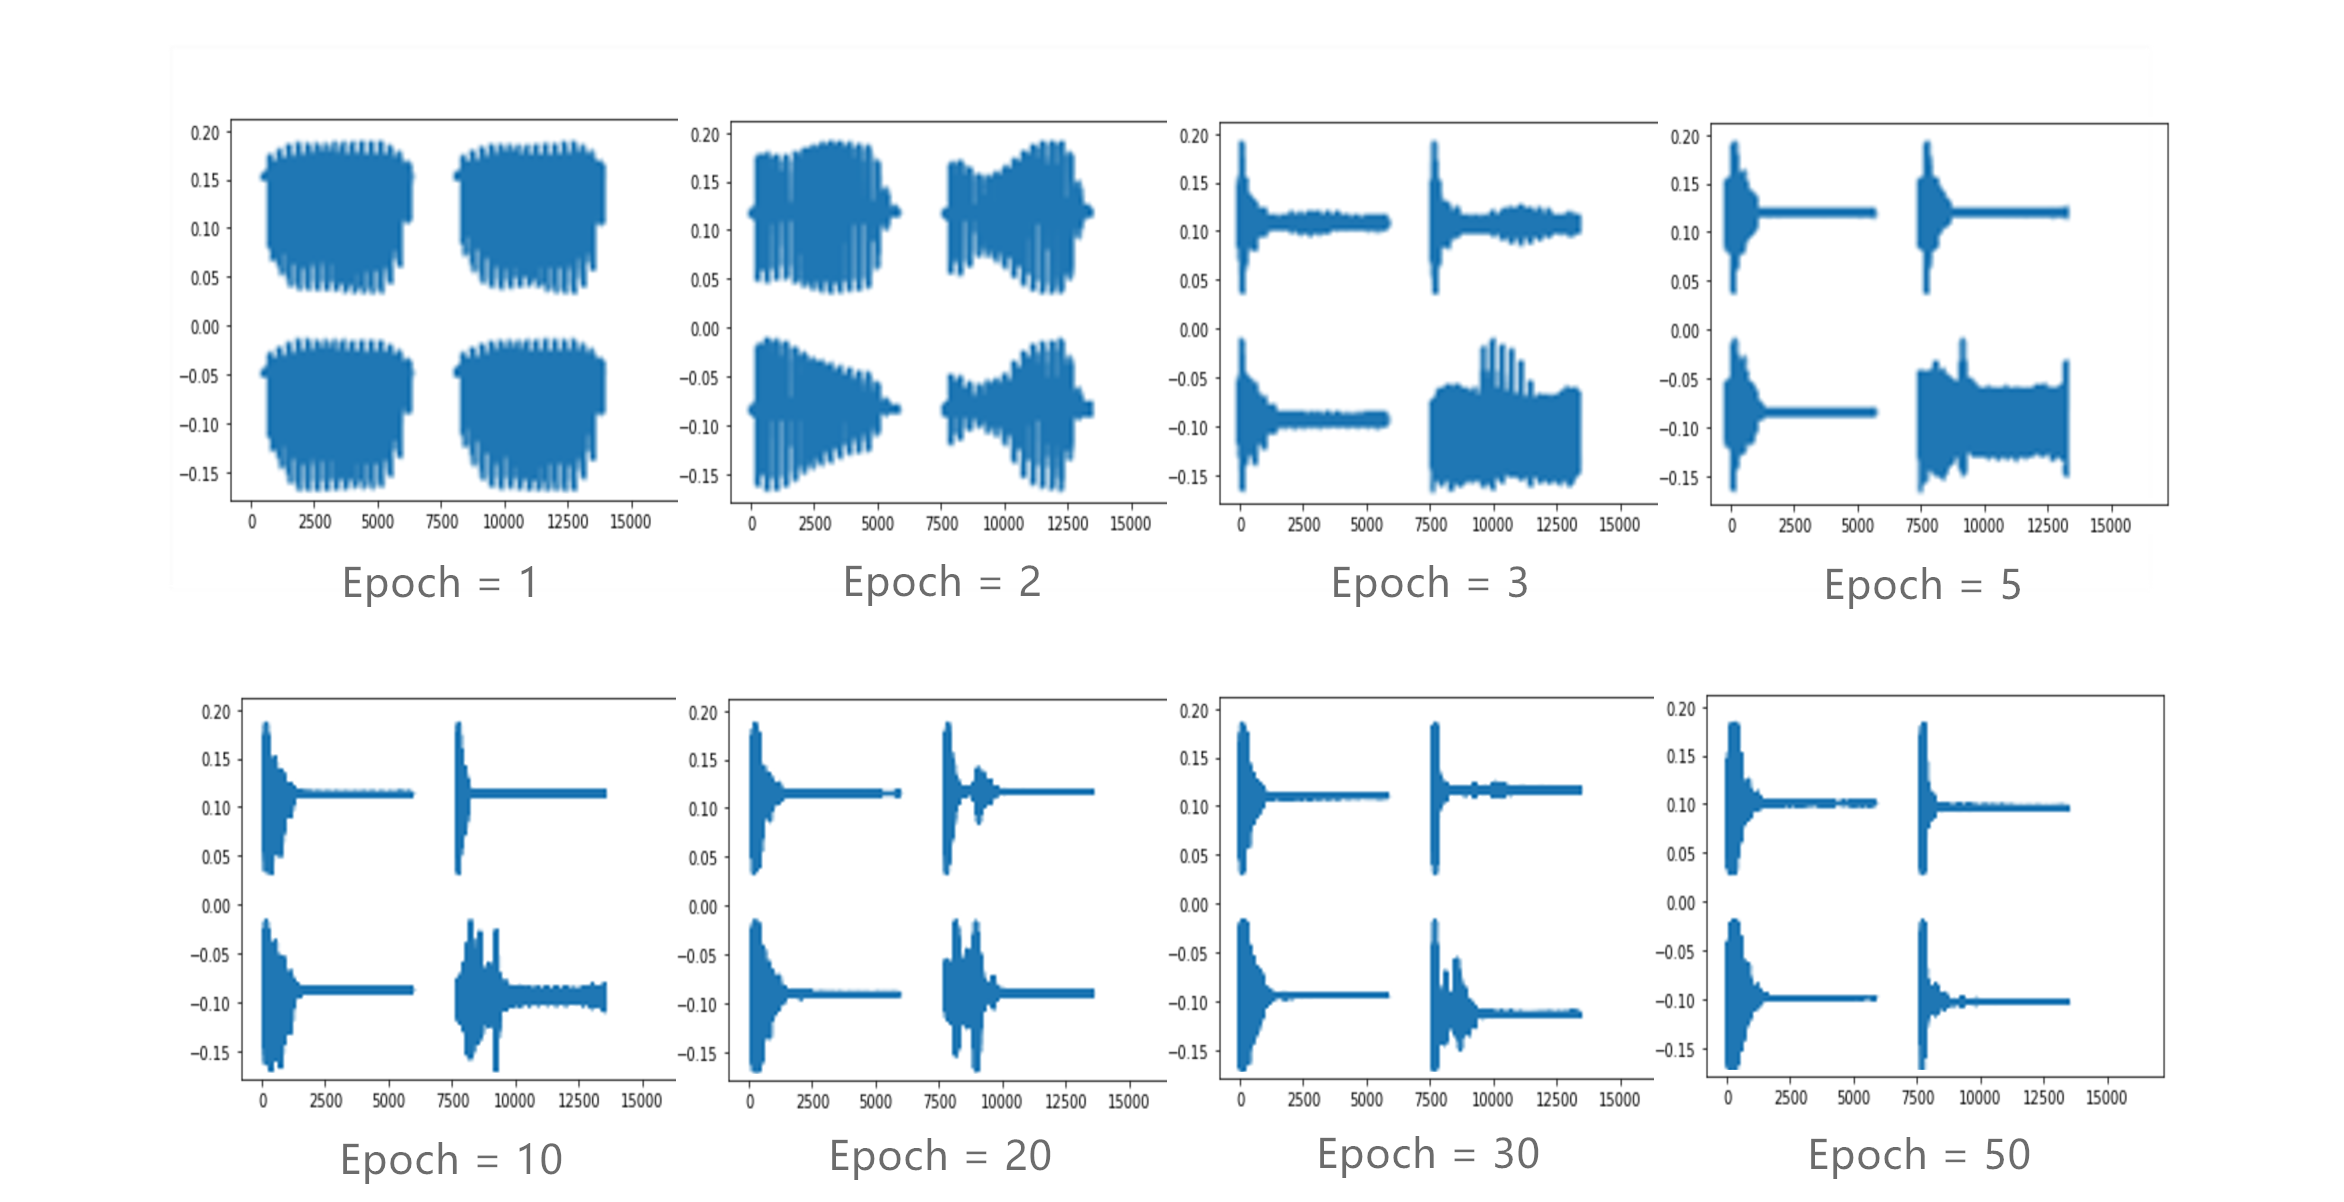
\includegraphics[width=1.0\textwidth]{image} 
\caption{Audio Waveform Images on the GAN learning the envelope of the sound}
\label{Fig.main2}
\end{figure}
Figure 1 shows the audio waveforms that the generator produced as the epoch increased from 1 to 50. When epoch is very small, the waveforms look like the noise wave, as it increases, the GAN gradually learns the envelope of the sound.   

To gain insight into how sounds generated by the trained model compare to the pre-trained model and the training dataset, we plotted a selection of samples in two dimensions based on sound similarity. To generate this plot, 100 samples were randomly selected from the training set and 100 samples were generated from the pre-trained model and the trained model. MFCCs were calculated on all audio files. For each frequency band, the mean and standard deviation was calculated to summarize time slices. Since the results of MFCC are a 40-feature vector for each audio signal, we decided to use principal component analysis (PCA) to perform dimensionality reduction. We reduce the dimensionality from 40 to 2, so that samples could be visualized on a 2D figure. The visualization is shown below. 

\begin{figure}[H] 
\centering 
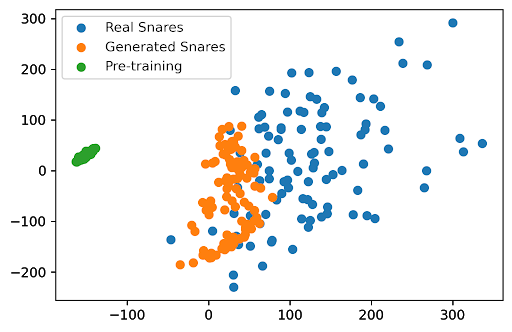
\includegraphics[width=0.7\textwidth]{unnamed} 
\caption{2D plot of pre-training audio, generated snares audio and  real snare audio}
\label{Fig.main2}
\end{figure}
In figure2, the X-axis is the first principal component and Y-axis is the second principal component. This plot shows how all the sounds from the pre-trained model are clumped together, and then after training have expanded towards the sonic distribution of the training snare drums. 


\newpage
\bibliography{csc503.bib}
\bibliographystyle{iclr2020_conference}

\end{document}
